\documentclass[12pt, a4paper]{article}
\setlength{\parindent}{0pt}
\usepackage{amsmath}
\usepackage{amsthm}
\usepackage{amssymb}
\usepackage{graphicx}
\usepackage[a4paper, portrait, margin=1in]{geometry}

\graphicspath{.}

% i like the black square better.
\renewcommand{\qedsymbol}{$\blacksquare$}
%\renewcommand{\implies}{\Rightarrow}

\newcommand{\N}{\mathbb{N}}
\newcommand{\ddx}{\frac{d}{dx}}

\newtheorem{theorem}{Theorem}

% let's begin
\begin{document}

\textbf{(Q2)}

In order to find and classify all critical points, we require the first
and second derivatives of $f$:

\begin{gather*}
    f'(x) = x^{2/5} - x^{-4/5}\\
    f''(x) = \frac{2}{5}x^{-3/5} + \frac{4}{5}x^{-9/5}
\end{gather*}

Solving $f$ and $f'$ for 0:

\begin{align*}
    f(x) = \frac{5}{7}x^{7/5} - 5x^{1/5} & = 0\\
    5x(\frac{1}{7}x^{2/5} - x^{-4/5}) & = 0 \implies x = 0\\
    \frac{1}{7}x^{2/5} & = x^{-4/5}\\
    x^{6/5} = (x^{3/5})^2 & = 7\\
    x^{3/5} & = \pm \sqrt{7}\\
    x & = \pm (\sqrt{7})^{5/3}\\
    \\
    f'(x) = x^{2/5} - x^{-4/5} & = 0\\
    x^{2/5} & = x^{-4/5}\\
    x^{6/5} = (x^{3/5})^2 & = 1\\
    x^{3/5} & = \pm 1\\
    x & = \pm 1
\end{align*}

Thus, $f$ has roots at $\pm(\sqrt{7})^{5/3}$ and $0$, as well as max/min points
at $\pm 1$.

Another thing to note is that $f'(x)$ is undefined at $x = 0$, so $f$ has a
vertical tangent line at $x = 0$.

Using $f''$ to determine concavity, we have:

\begin{align*}
    f''(1) & = \frac{2}{5}(1)^{-3/5} + \frac{4}{5}(1)^{-9/5} = \frac{6}{5} > 0\\
    f''(-1) & = \frac{2}{5}(-1)^{-3/5} + \frac{4}{5}(-1)^{-9/5} = - \frac{6}{5} < 0
\end{align*}

So $f$ is concave up at $x = 1$ and concave down at $x = -1$, so its maximum
point is at $x = -1$ and its minimum point is at $x = 1$.

With all this information, we can then sketch the graph of $f$:

\begin{center}
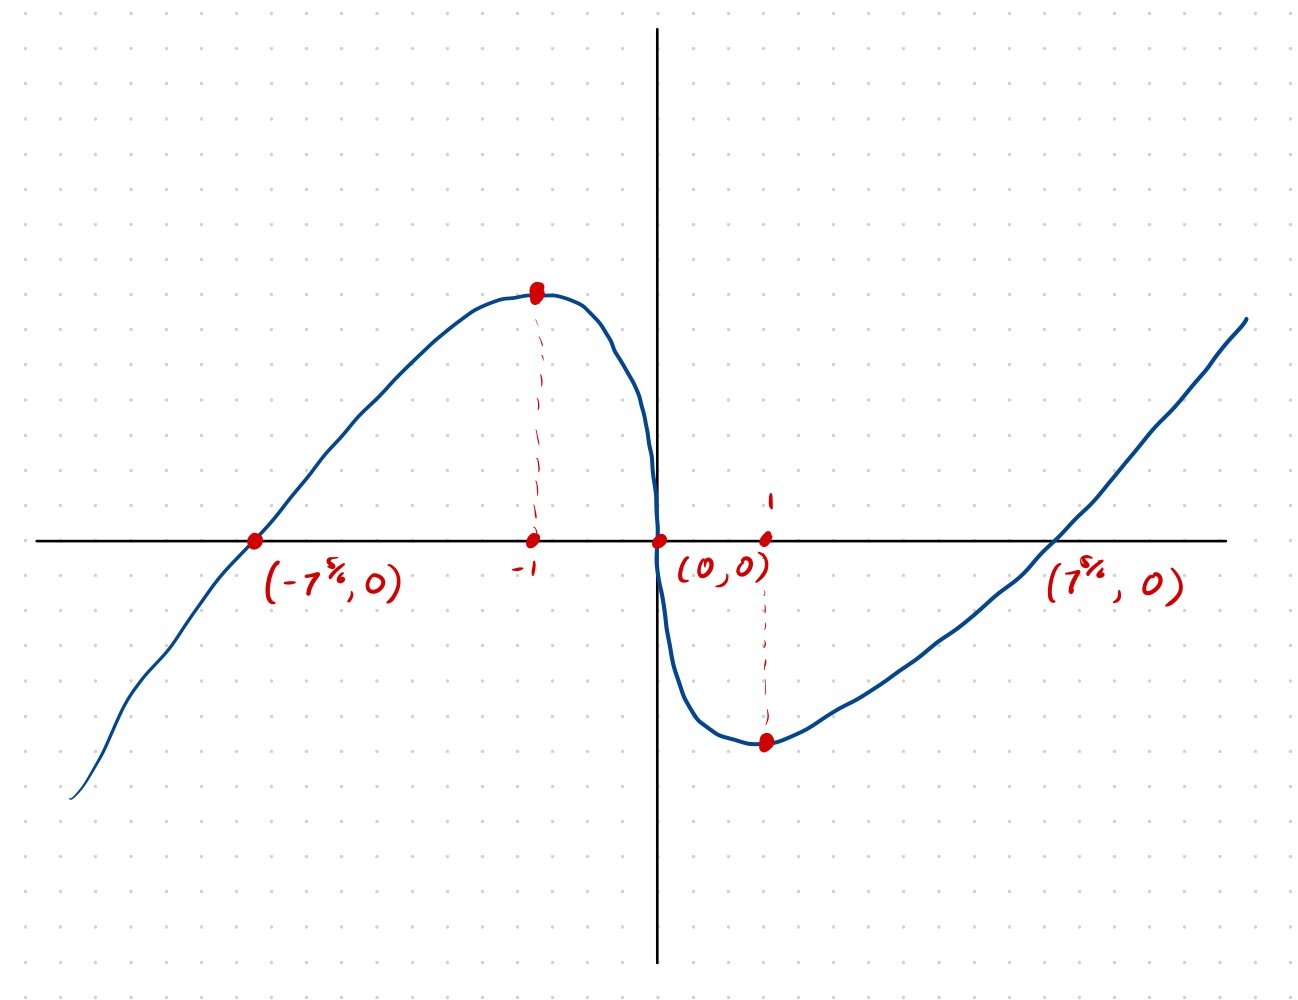
\includegraphics[width=15cm]{q2_sketch.JPG}
\end{center}

\end{document}